\documentclass[11pt,a4paper]{article}

\usepackage{blindtext}
\usepackage{booktabs}
\usepackage{pgfplots}
\usepackage{marginnote}
\usepackage{tabularx}
\usepackage[marginparwidth=2.3cm]{geometry}
\usepackage[ampersand]{easylist}

\date{\today}

\title{L2 Physics Notes}
\author{Ben Tomlin}

\begin{document}
\maketitle

\begin{abstract}
This document is a overview of and reference for the physics concepts and the mathematical equations that describe them. 
\end{abstract}


\tableofcontents

\part{Motion}

\section{Motion}
Describe motion of objects in two dimensions.

\begin{description}
	\item[Vectors] Vectors, a direction and size. Addition and subtracting. Components.
	\item[Forces] Forces. How they produce an acceleration. Newtons laws.
	\item[Displacement, Velocity, Acceleration] Used to describe an objects motion.
	\item[Relative Velocity] Describing an objects velocity as seen by a moving observer. 
\end{description}

\subsection{Kinematic Equations}
\marginnote{\textbf{constant} means unchanging. Is a stationary objects acceleration constant?}
The kinematic equations describe motion of an object that has a constant acceleration. \\


When an object is accelerating over a time period, its velocity will change between the start of that time period and
the end (unless acceleration is zero). Also, the object will travel some distance during this time. Kinematic
equations relate these quantities. \\

\reversemarginpar 
\marginnote{
	\textbf{averaged} means that the quantity sits at an average value. At a given instant though, it may be greater or
	lesser than the average\\

	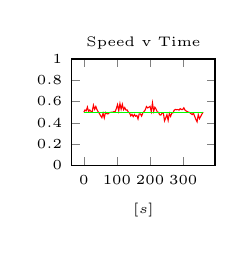
\begin{tikzpicture}
		\begin{axis}[
			xlabel={[$s$]},
			title={\tiny Speed v Time},
			tiny,
			ymin=0,ymax=1,
			width=3.4cm,
			legend style={nodes={scale=0.7}}
		]
		\addplot[
			domain=0:360,
			samples=100,
			color=red,
		] {0.5+0.1*rnd*sin(x*4)};
		\addplot[
			domain=0:360,
			samples=2,
			color=green,
		] {1/2};
	\end{axis}
\end{tikzpicture}
}
\normalmarginpar
Importantly, they are used only when acceleration is \textbf{constant} or \textbf{averaged}. \\

\noindent
\begin{tabular*}{\columnwidth}{|c l @{\extracolsep{\fill}} c|}
	\toprule
\textbf{Symbol} & \textbf{Meaning} & \textbf{[Unit]} \\ \midrule
	\(V_i\) & Initial velocity. The velocity at the beginning of a time period. &\(ms^{-1}\) \\
	\(V_f\) & Final velocity, or the velocity at the end of a time period. & \(ms^{-1}\) \\ 
	a & Constant (or average) acceleration for the time period. & \(ms^{-2}\) \\
	t & Time period over which velocity canged. & \(s\) \\
	d & Distance that the object travel(s,led) (in the time period) & m \\ \bottomrule
\end{tabular*}

\noindent
\begin{tabular*}{\columnwidth}{|c@{\extracolsep{\fill}}ccc|}
	\hline
	\Large $V_f=V_i+at$ & $d=\frac{V_i+V_f}{2}t$ & $V_f^2=V_i^2+2ad$ & $d=V_it+\frac{at^2}{2}$ \\
	\hline
\end{tabular*}

\part{Forces}

\part{Energy}

\part{Momentum}

\end{document}
